\section{Current status}

In this chapter, the openness status of the SSDI will be analyzed by applying this Open SDI Assessment Framework. It acts as a snapshot of the current state of affairs. Most information regarding the current status, scores \& commitments of the SSDI has been gathered using and analysing the Scottish data portal, the statements within their own documentation and the Open Government Partnership analysis 
\citep{ssdi,ssdi_documentation,opengovpartnership_mainpage}.

The Open Government Partnership scores the openness of countries based upon a number of useful criteria, such as level of ambition, level of user participation, and if they actually went through and succeeded on their promises. These scores were used to judge the Scottish NSDI, even though the general state of Open Government within Scotland does not necessarily correlate to the state of the NSDI in particular. This is because it is implied that these documents regard government data as being the super-set of spatial data. \citep{opengovpartnership_increasing_participation, opengovpartnership_openpolicymaking}.

The Registers of Scotland (RoS) \citep{ros}, and their Land Information Service (ScotLIS), are used to analyse the quality of the parcel dataset. 

\begin{figure}
    \hspace*{-3cm}
    \graphicspath{ {images/} }
    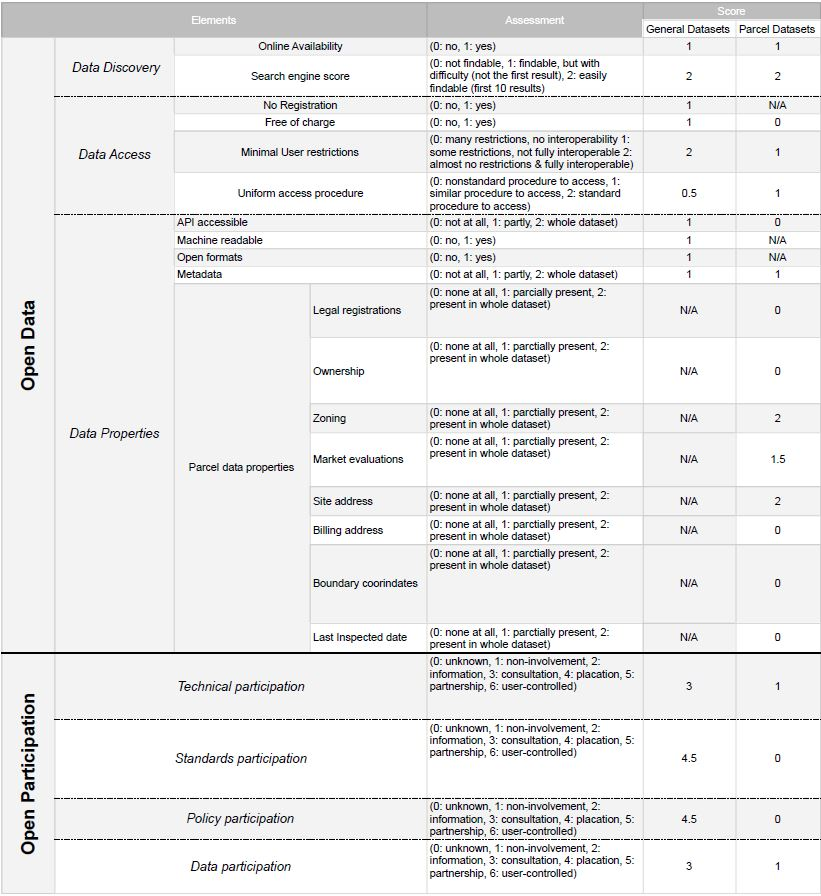
\includegraphics[width=20cm]{images/assessment_framework_assessment.JPG}
    \caption{Assessment results}
    \label{fig:assesment_result}
\end{figure}

The overall results of the assessment framework can be visualized in Figure \ref{fig:assesment_result}. The overall analysis, as well as the justification of the scoring are presented in this chapter.

Throughout this assessment, a common theme will become apparent, namely the fact that different data platforms, provided by either the government, or local municipalities, or national agencies (Registers of Scotland) differ vastly in accessibility and how their data is presented.

\subsection{Open Data}

\subsubsection{Data Discovery} %DONE?

The Scottish government provides an online geoportal \citep{ssdi}, which includes around 800 datasets and 130 services, which can be divided into either INSPIRE themes or general topics, such as environment, inland waters or geoscientific information. The website seems easy to use, and searching for data on this platform is relatively simple. The data itself can be either downloaded or visualized on the map which is built into the platform itself. 
However, some of the data does not seem to be well maintained. For example, when searching for the road network database, neither the Scottish geoportal, nor the publishing agency (in this case Transport Scotland) or the data portal which covers the entire United Kingdom had an available link for download of this data. All of these different sources are broken, possibly due to a lack of maintenance.

The parcel data is available on another website, namely the ROS \citep{ros} . It does take a considerable number of clicks, but (basic) parcel data can be visualized on this platform.

Overall, the data is indeed discoverable, even if it has certain issues. For this category, our grading is "1-discoverable", and the problems mentioned will be discussed in further detail later in this chapter.

\subsubsection{Search engine score}

When using the Google search engine, a typical search like "Spatial Data Scotland" yields the SSDI as the first result. The Portal is thus very findable. Same goes for the parcel data, when searching on Google, the portal itself is amongst the top results. Thus, this category receives a "2-easily findable" score for both types of datasets.


\subsection{Data Access}

\subsubsection{No registration}

The Spatial Data portal does not require the user to login in order to download any of the datasets which are available on the website. In fact, the only accounts which can be created on the platform are government-owned (i.e. the data providers), which can add or modify existing metadata.

There are a number of various different data platforms, mostly focused on individual municipalities (such as Aberdeenshire Council Open Data, Dundee Open Data Portal, and so on), which also offer users the option to download the datasets which are available on these websites without having to create an account. Registering to the platform gives third-party stakeholders the ability to follow already-available datasets or to submit data requests \citep{dundee_data_portal}.

For these reasons, we consider that spatial data which covers the Scottish territory is available without registration, thus it receives a score of "1 - yes"

The Land Register doesn't offer the possibility for registration, so this criterion does not apply for parcel data, so scoring this section is not possible (thus, not applicable, or N/A in Figure \ref{fig:assesment_result})

\subsubsection{Free of charge}

All datasets on the Scottish Data portal are free of charge (score: "1 - yes").

The web-viewer of the RoS can also be used free of charge. The actual fees for registering a change of ownership however, is not. This fee scales by parcel value. (score: "0 - no")


\subsubsection{Minimal User restrictions} % Jos

The UK Government Licensing Framework provides the framework which encompasses the recent open government \& PSI directive developments \citep{national_archives_ukglf}. It contains two main components, the Open Government Licence (OGL), and the Crown copyright. The OCL is a lenient licence which actively promotes the use and reuse of data. It offers no international boundaries, and is internationally inter-operable \citep{national_archives_ukglf_opengov}. The Crown Copyright states that even though use \& reuse is promoted, the Crown is still the final copyright holder of the data. 

All spatial datasets present in the NSDI are OCL licenced and copyrighted, so it is fair to say that the NSDI as a whole offers little to no user restrictions. 

The Registry of Scotland also falls under the Crown copyright \& OGL licence, but do not clearly state the usability of their data: "Material on this site is protected by Crown copyright unless otherwise indicated. It can only be used under the OGL. Where we identify any material as the copyright of a third party, you'll need the copyright holder's permission to reproduce that material." \citep{ros_crown_copyright}. We can at least state that the RoS is not actively promoting the reuse of their data, and make it harder for users to determine if they are allowed to do so. They will thus score lower on the criteria of minimal user restrictions. 

\subsubsection{Uniform access procedure}

The procedure used to access the data is far from standard on the different platforms. For example, on the official spatial data platform, finding and downloading datasets is relatively straightforward. The local governments' websites vary as well, some are easier to access than others.

On the other hand, the Registers of Scotland proved challenging. When looking on the ROS platform, we had a difficult time trying to find and access the parcel information, and we believe that an inexperienced used would have an even more difficult time. 

For this criteria, our assessment is between 0 and 1 for the general datasets, due to the variety of available platforms, and 1 for the RoS.

\subsection{Data Properties} %Alex

\subsubsection{API accessible} %Alex

The national spatial data portal does offer the possibility to access the catalog using a GeoNetwork REST API \citep{ssdi_api}, which is still in a beta version (0.1, so this project is either just being launched, or not maintained). The terms of service of this API are inaccessible, so our assessment is that this service exists but its maintenance is not a priority of the agency. In contrast, the main data-platform for the entirety of the United Kingdom offers a well documented API.

The portals of the municipalities don't offer the possibility to use an API at all, and neither does the ROS agency for parcel data. Thus, for this section, we will grade it with "1 - partly" for general datasets, due to lack of maintenance, and "0 - not at all" for the parcel datasets

\subsubsection{Machine readable} %Alex

In general, data portals (be them on the national level or municipality level) do offer the datasets in different machine readable formats, such as CSV, XLS, JSON, GeoJSON, XML or KML. Certain platforms also offer the possibility to download or search (using the SPARQL query language) the data in the RDF standard, which facilitates integration in other Semantic Web systems.

The machine readable criterion is not applicable for the parcel data, as this is not available to download, and can only be visualized on the ROS platform.

Certain platforms also offer the possibility to access the datasets using Web Map Services, which makes it even easier for developers to create pieces of software which utilize this data.

\subsubsection{Open Formats} %Alex

As mentioned in the previous point, the formats which are used, which allow the data to be machine readable, are also open. 

\subsubsection{Metadata}

From our analysis, while some datasets contain extensive Metadata, others do not offer any at all. This is usually the case for smaller platforms, from the municipalities. The main Scottish geo-portal, on the other hand, contains a very well documented and complex metadata for the datasets which are available. 

The Scottish SDI fully complies to the UK-GEMINI standard for meta-data in the UK. This is the UK's Translation of the INSPIRE directive \citep{ssdi_documentation}. 

\subsubsection{Parcel Data Properties} 

Legal registrations - Not open (score 0)

Ownership - No information regarding who owns a certain property is available for free (score: 0)

Zoning - Whether a property type is residential, commercial, land, agriculture, forestry or other can be seen directly on the platform. (score: 2)

Market Evaluations - Historical prices of the property are visible when looking at a certain parcel. However, sometimes, only older evaluations are displayed, and newer ones (from the last 5 years) are restricted, with the mention that the price is included in the property documents. (score 1.5)

Site address - Given that a parcel can only be visualized/accessed on the basis of an address, a certain parcel also has an address attached to it (score 2)

Billing address - Not mentioned (score 0)

Boundary coordinates - The boundary coordinates are displayed on the ROS platform, but downloading them is not possible (or viewing the exact coordinates, for that matter). 

Last Inspected date - Not available (score 0)

\subsection{Open Participation} %Jos

Before going in-depth into each element, it should be noted that, as compared to the other geographical datasets, the ROS remains unclear on their levels of public participation. It seems this HVD is maintained exclusively by the Scottish authorities, but more research is needed to confirm this. 

\subsubsection{Technical}
The level of technical participation is limited. While the SSDI is officially provided by the Scottish government as 'data controller', the actual hosting and management is done by 'data processor' Astun Technology, a commercial party with a commitment to Open Source development \citep{ssdi_documentation}. While this means that technical user participation might become viable in the future through the means of open source participation \citep{osi_definition}, right now, users with technical knowledge cannot contribute besides suggestions \& feedback. 

From these IRM evaluations and the statements of the SSDI, we conclude that the difference in attention to the creation of visions, plans \& policies compared to the actual progress being made, is reflected in the levels of user participation present in Standards \& Policy making versus Technical \& Data participation. 

\subsubsection{Standards \& Policy}

% add this: 
% https://opendatabarometer.org/country-detail/?_year=2017&indicator=ODB&detail=GBR

The second component of an Open SDI is open participation. The Open Government Partnership offers, among other information, a timely and precise assessment regarding participation on their website \citep{opengovpartnership_mainpage}. The Government of Scotland appears very committed to open government plans, visions and strategies since 2016. The Open Government page on Scotland states that both in the development \& implementation phase, independent user participation was granted in the form of consultation \& forum, and that these where open to any party interested. 

According to Independent Reporting Mechanisms (IRMs), Scotland's commitments are both ambitious and relevant to Open Government initiatives \&  \citep{opengovpartnership_increasing_participation, opengovpartnership_openpolicymaking}. However, the level of completion of these commitments vary from moderate to substantial progress, and none of the commitments have been fully completed yet. Still, the policies brought forward by the Open Government Partnership Action Plans themselves have been made using citizen partnership \citep{opengovpartnership_action_plan}. This is why the level of Policy \& Standards participation is scored with a 4.

\subsubsection{Data}
Currently, there is no self-registration available on the SSDI \citep{ssdi_documentation}. To become a contributer of data to the SSDI, one has to mail SpatialData.gov.scot directly, and ask them for permission. The docs also state that "Currently, user accounts are created for organisations as a whole rather than individuals." \citep{ssdi_documentation}. This means that there is data participation from multiple organizations, but only to a limited extend.

% All Action plans
% https://www.gov.scot/publications/open-government-partnership-scottish-action-plan/
% https://www.gov.scot/publications/scotlands-open-government-action-plan-2018-20/
% https://www.opengovpartnership.org/members/scotland-united-kingdom/
% https://www.opengovpartnership.org/members/scotland-united-kingdom/commitments/SCO0005/
% https://www.opengovpartnership.org/members/scotland-united-kingdom/commitments/SCO0007/
% https://www.gov.scot/policies/community-empowerment/
% https://www.gov.scot/publications/fairer-scotland-action-plan/
